% Adjusting chapter title format for regular (numbered) chapters
\titleformat{\chapter}[display]
  {\normalfont\huge\bfseries\centering}{\chaptertitlename\ \thechapter}{20pt}{\Huge}

% Using similar styling for unnumbered chapters but without "Chapter" prefix
\titleformat{name=\chapter,numberless}
  {\normalfont\huge\bfseries\centering}{}{0pt}{\Huge}

\titlespacing*{\chapter}{0pt}{50pt}{40pt} % Adjust vertical spacing before and after the title

\chapter{Introduction} % Ensures chapter numbering starts correctly

\section{Background and Motivation}

Deep Neural Networks (DNNs) are increasingly being used in diverse applications due to their ability to match or exceed human-level performance. With the broader deployment of DNNs in various safety-critical systems like autonomous vehicles, healthcare, and avionics, concerns over their safety and trustworthiness have been raised \cite{ZhaoXBanks}. The availability of large datasets, fast computing methods, and their high performance has enabled the use of DNNs in safety-critical applications \cite{LeCun}. The critical nature of such applications makes it essential to thoroughly evaluate these DNNs before deployment to guarentee their reliability and safety.


In recent years, there has been significant amount of publications focused on tackling this concern. Figure. \ref*{fig:no_publish} visualizes the significant growth in the number of published papers related to DNNs safety from 2008 to 2023. The data is gathered using a comprehensive set of relevant keywords \footnote{The keywords used for data extraction include: 'deep neural network safety,' 'DNN verification,' 'DNN testing,' 'deep learning robustness,' 'neural network adversarial attacks,' 'DNN defense mechanisms,' 'DNN interpretability,' 'deep learning certification,' 'neural network validation,' and 'machine learning security.'}.

\begin{figure*}
  \centering
  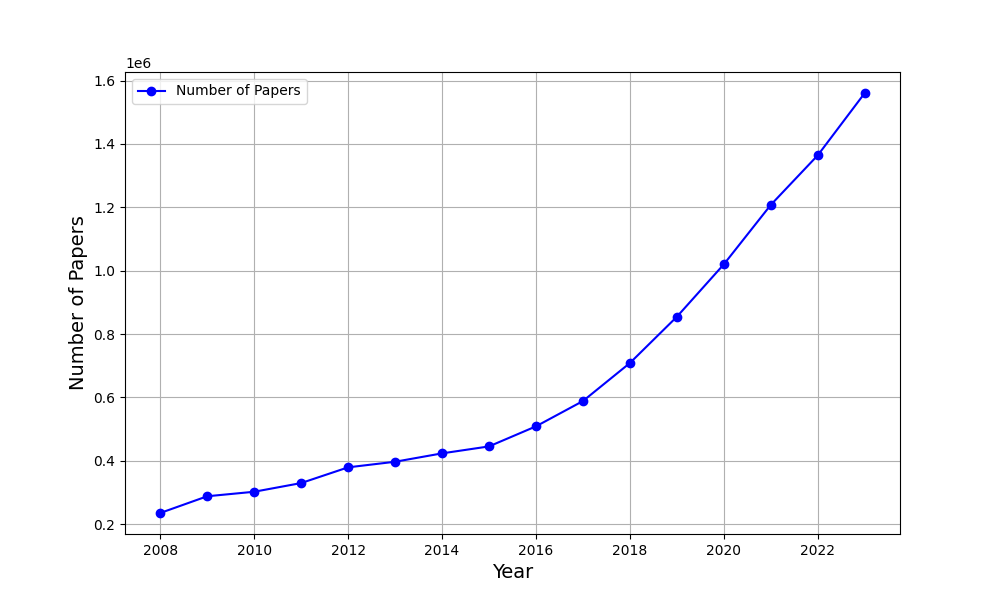
\includegraphics[width=\linewidth]{Number of Published Papers on DNN Safety.png}
  \caption{Number of Published Papers on DNN Safety}
  \label{fig:no_publish}
\end{figure*}

An important requirement for DNNs is that they are robust against input perturbations \cite{HuangX}. 
DNNs have shown a lack of robustness due to their vulnerability to adversarial examples, where even minor modifications to an input, sometimes imperceptible to humans, can destabilize the neural network  \cite{Goodfellow,Carlini}. Unlike traditional software, DNNs do not have a clear \hyperref[gloss]{\textsc{control-flow structure}} \label{Control-Flow Structure}. They learn their decision policy through training on large datasets, adjusting parameters gradually using various methods to achieve the desired accuracy. Consequently, traditional software testing methods like \hyperref[gloss]{\textsc{functional coverage}} \label{Functional coverage} and \hyperref[gloss]{\textsc{branch coverage}} \label{Branch coverage}  cannot be applied to DNNs, thus challenging their use in safety-critical applications. This is because DNNs lack explicit paths and branches that can be directly tested; their behavior emerges from complex interactions within their learned parameters, making it difficult to apply traditional coverage metrics that rely on predefined control flows \cite{Sekhon}.


In the past, researchers have extensively discussed both verification and testing techniques, which are useful for evaluating the DNNs. Verification involves proving the \hyperref[gloss]{\textsc{property}} \label{property} of a system through mathematical proof. This approach ensures that certain property is met by the system based on a \hyperref[gloss]{\textsc{formal analysis.}} \label{formal analysis} However,DNN verification techniques are promising, they suffer from a scalability problem, due to the high computational complexity and the large size of DNNs. Up to now, DNN verification techniques either work with small scale DNNs or with approximate methods with convergence guarantees on the bounds \cite{HuangX}. This limitation impacts the ability to achieve high coverage, which means thoroughly testing the model across a wide range of input scenarios and conditions to ensure that all potential issues are identified.

On the other hand, testing focuses on identifying defects (i.e, counter example to a property) or provide assurance cases \cite {Rushby}, by evaluating the behavior of system through {\textsc{empirical methods.}} \label{empirical methods} As a result, they can achieve high coverage, which suggests that more of a DNN's behavior has been tested and therefore the DNN has a lower chance of containing undetected bugs \cite{HuangX}. While these coverage metrics are useful, they often fall short in providing comprehensive evaluations. This is because they primarily focus on the internal structure of the deep models, such as neuron activation patterns, rather than evaluating the DNNs behavior on a diverse set of inputs. This internal focus can miss identifying specific inputs that cause failures or unexpected behavior.


\begin{tcolorbox}[colback=purple!2!white, colframe=purple,title= Thesis Goal]

    The primary aim of this thesis is to examine existing testing methods to check the robustness of DNNs, identify opportunities for improvement, and highlight the need for a fast, scalable, generalizable end-to-end testing method.
    \end{tcolorbox}
    



% \textcolor{olive}{ \textbf{Solution:} To address these limitations, I propose a complete framework that encompasses the entire process from specification to error summarization. This framework will introduce new coverage criteria driven by specific requirements and based on both local and global correctness. Local correctness involves evaluating the AI subsystem's performance on individual inputs representing specific classes, subjected to various transformations, ensuring that the model remains robust under specific conditions. Global correctness assesses the overall behavior of the AI system across a comprehensive range of scenarios, ensuring holistic robustness and reliability. By focusing on testing with specification-driven criteria, my approach aims to provide immediate feedback and uncover a wide range of issues, enhancing the robustness of DNNs.}



\section{Research Goal}

 The primary goal of this research is to enhance the robustness of DNNs used in safety-critical systems. To accomplish this, a detailed and comprehensive testing framework will be developed and implemented. This framework will formalize and utilize specifications related to various aspects of the pre-trained DNN model, such as model architecture, including the number of layers, types of layers (e.g., convolutional, recurrent), number of neurons per layer, weights, and activation functions. Additionally, it will consider input data characteristics, including the type (e.g., images, text), size (e.g., number of samples), and format (e.g., resolution, encoding), as well as operational conditions, such as expected input ranges and environmental factors (e.g., brightness, noise, rotation, fog). User requirements, like specific modules to test or critical scenarios to focus on, and evaluation metrics (e.g., accuracy, precision, recall) will also be incorporated.

If no specific requirements are provided by the user, the framework will operate based on default parameters to ensure a thorough assessment. However, it can also be customized for specific cases or multiple cases based on user specifications. For instance, a user might require the framework to focus on a particular class or scenario that is critical. This flexibility ensures that the framework addresses the most important aspects of the application in question.

To accurately identify weaknesses and areas for improvement, the framework will calculate both local coverage and global coverage using probabilistic programming language. This approach allows for a detailed analysis of the model's behavior under different conditions, providing insights into how the model performs in specific scenarios and overall. By examining local-level coverage, the framework can detect vulnerabilities that may arise in specific parts of the model or under particular conditions. Global-level coverage assessment, on the other hand, evaluates the model's overall stability across a wide range of scenarios. Together, these analyses help pinpoint specific vulnerabilities and highlight areas where the model can be improved, ultimately leading to more robust systems.

Additionally, the framework will generate a comprehensive error summary, providing insights into the types and frequencies of errors encountered. This summary will highlight critical failure points and suggest targeted improvements, enabling developers to enhance the system robustness.
Through continuous evaluation and iterative refinement, the framework aims to significantly enhance the safety and dependability of DNN models across different operational levels. This ongoing process ensures that the models remain robust and effective in a wide variety of real-world applications, ultimately contributing to their reliability in safety-critical systems.

\subsection{Research Gap}
Currently, there is no end-to-end automated framework that thoroughly integrates data, test cases, and test coverage according to given specifications and provides a detailed error summary.

\subsection{Research Objectives}
The objectives of this research are to:

\begin{enumerate}
    \item \textbf{ User-defined specifications:} Formalize specifications by developing templates and a specification language that enable users to clearly define and specify the properties of the system and its associated data for testing purposes.
    \item \textbf{Design framework:} Create a framework that test the DNN under a variety of conditions, ensuring it meets performance standards even in edge cases and adverse scenarios.
    
    \item \textbf{Efficient input sampling:} Develop a sampling approach that effectively identifies and prioritizes corner cases. It can be used to guide best selection of inputs for test case generation.
  
    \item \textbf{Effective test case generation with interpretability analysis:} Implement interpretability analysis to identify and prioritize key influential features in the DNN testing process, exploring the use of high influential features for effective test case generation.
    
    \item \textbf{Systematic robustness evaluation:} Integrate advanced probabilistic methods to evaluate both \hyperref[gloss]{\textsc{\textsc{local coverage}}} \label{Local coverage}  and \hyperref[gloss]{\textsc{\textsc{global coverage}}} \label{Global coverage}, providing comprehensive error summaries and \hyperref[gloss]{\textsc{systematically}} \label{systematic}  assessing robustness at different levels within the framework.
    
    \item \textbf{Quantifying model robustness through error summarization:} Innovate error summarization techniques that identify and quantify model weaknesses, utilizing error summarization to quantify the impacts on model robustness.
\end{enumerate}

\subsection{Research Questions}

\begin{enumerate}
  \item How can we design a \hyperref[gloss]{\textsc{comprehensive}}\label{comprehensive} framework to test system robustness?
    \item How can we clearly define and specify the properties of the system?    
    \item How can we sample inputs efficiently?
    \item How can we generate highly effective test cases that ensure complete coverage?                                                                                                                                                     
    \item Can interpretability analysis aid in effective test case generation?
    \item How can we ensure comprehensive test coverage for deep learning models?
    % \item How can comprehensive coverage criteria be designed and implemented to systematically evaluate the robustness of deep learning models?
    % \item Can SHAP values be used for effective test case generation? 
    % \item How can we \hyperref[gloss]{\textsc{systematically}} \label{systematic}  evaluate the robustness both at local (property-specific) and global (overall system) levels within the framework?
    \item How can error summarization be employed to quantify the impacts on model robustness?
      
    % \textit{Research Objective:} Develop a hybrid sampling approach that effectively identifies and prioritizes corner cases.
        

       
    %  \textit{Research Objective:} Create a robust framework that systematically evaluates DNN performance, reliability, and robustness.
    
    
 
    % \textit{Research Objective:} Integrate advanced probabilistic methods to evaluate both local and global robustness, providing comprehensive error summaries.
        
        

    % \textit{Research Objective:} Implement SHAP analysis to identify and prioritize key influential features in the DNN testing process.
       
    
  
    % \textit{Research Objective:} Innovate error summarization techniques that identify and quantify model weaknesses.

\end{enumerate}


\section{Research Contribution}

This research makes the following key contributions to the field of deep learning correctness evaluation:

\begin{itemize}
    \item An \textit{\textcolor{blue}{end-to-end pipeline}} is designed for evaluating the robustness of the system.
    \item A \textit{\textcolor{blue}{hybrid sampling}} technique is proposed to identify and prioritize the corner cases.
    \item A \textit{\textcolor{blue}{conceptual framework}} is proposed that quantifies both local and global robustness. This framework uses Problog, a probabilistic logic programming language, to verify system robustness. This approach allows for more precise and reliable robustness verification.
    \item An \textit{\textcolor{blue}{interpretability-driven test case generation}} approach is employed to pinpoint critical input features, which are then used to create test cases with a higher probability of inducing mispredictions, thus effectively evaluating and enhancing model robustness.
    % \item A novel \textit{error summarization} approach is introduced, which helps in better identifying where model makes mistakes, especially in relation to specific classes and property.
    \item All \textit{\textcolor{blue}{experiments}} are conducted using publicly available datasets, including DAWN, CIFAR, and MNIST.
\end{itemize}

\begin{center}
    \fcolorbox{gray}{lightgray}{
    \parbox{0.95\linewidth}{
    \textbf{Note:} The current contributions do not include methods for defining system properties and error summarization techniques. Additionally, adversarial examples used in the experiments are taken from existing literature.
    }
    }
    \end{center}
\section{Organization of the Thesis}\hypertarget{organization of thesis}{}
The remainder of the thesis is organized as follows: related studies are presented in Chapter \ref{chp:2}. The system model and proposed methodology are demonstrated in Chapter \ref{chp:3}. Chapter \ref{chp:4} describes the simulation results of our proposed schemes. Finally, the findings of this work along with future directions are presented in Chapter \ref{chp:9}.




\clearpage
